
\documentclass[12pt]{article}
\usepackage{times}
\usepackage{setspace}
\setstretch{1.5}
\usepackage{amsmath,amssymb, amsthm}
\usepackage{graphicx}
\usepackage{bm}
\usepackage[hang, flushmargin]{footmisc}
\usepackage[colorlinks=true]{hyperref}
\usepackage[nameinlink]{cleveref}
\usepackage{footnotebackref}
\usepackage{url}
\usepackage{listings}
\usepackage[most]{tcolorbox}
\usepackage{inconsolata}
\usepackage[papersize={8.5in,11in}, margin=1in]{geometry}
\usepackage{float}
\usepackage{caption}
\usepackage{esint}
\usepackage{url}
\usepackage{enumitem}
\usepackage{subfig}
\usepackage{wasysym}
\newcommand{\ilcode}{\texttt}
\newcommand{\p}{\partial}
\usepackage{etoolbox}
\usepackage{physics}
\usepackage{xcolor}
\patchcmd{\thebibliography}{\section*{\refname}}{}{}{}



\makeatletter
\renewcommand{\@seccntformat}[1]{}
\makeatother

\begin{document}



\title{\textbf{CSDS 440: Assignment 6}}

\author{Shaochen (Henry) ZHONG, \ilcode{sxz517} \\ Mingyang TIE, \ilcode{mxt497}}
\date{Due on 10/16/2020, submitted \textcolor{blue}{early} on 10/09/2020 \\ Fall 2020, Dr. Ray}
\maketitle


% % % % % % % % % % % % % % % % % % % % % % % % % % % % % % % % % %
% % % % % % % % % % % % % % % % % % % % % % % % % % % % % % % % % %
% % % % % % % % % % % % % % % % % % % % % % % % % % % % % % % % % %
\section{Problem 23}

\subsection{(i, ii, iii)}

\begin{figure}[H]
\minipage{0.32\textwidth}
  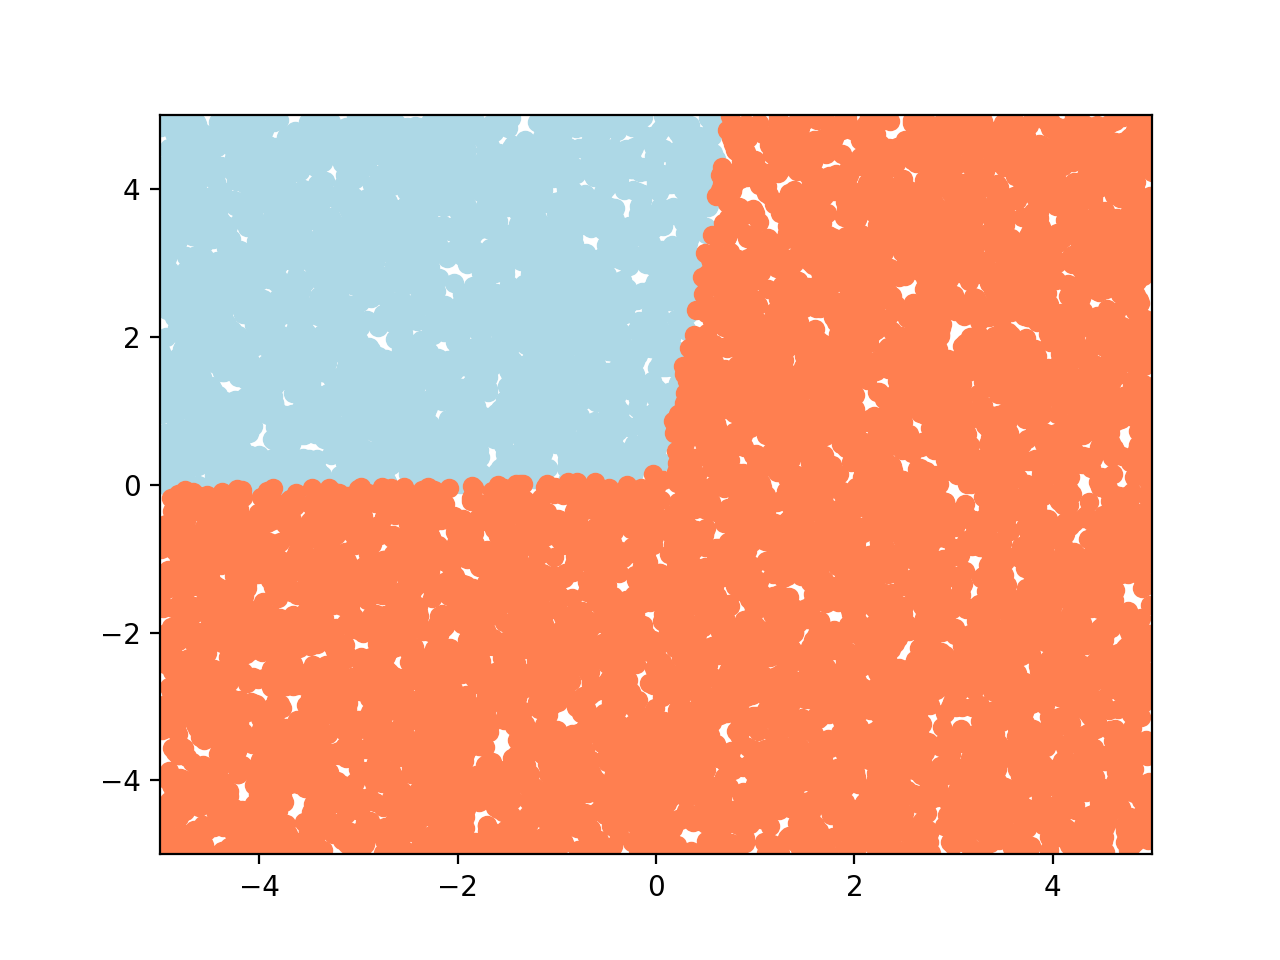
\includegraphics[width=\linewidth]{fig/fig_p23_1.png}
  \caption{$w \in [-10, 10]$}
\endminipage\hfill
\minipage{0.32\textwidth}
  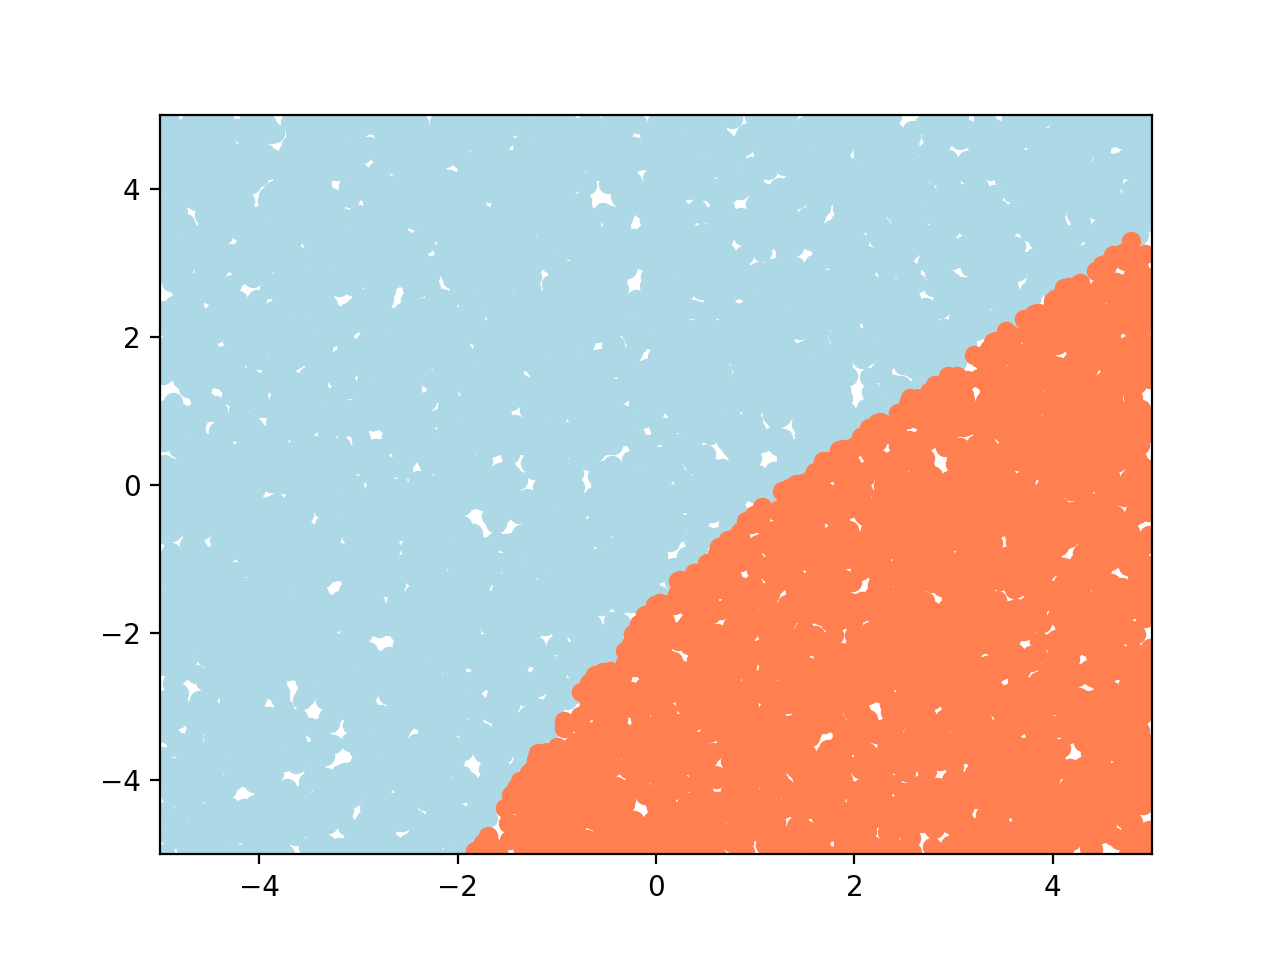
\includegraphics[width=\linewidth]{fig/fig_p23_2.png}
  \caption{$w \in [-3, 3]$}
\endminipage\hfill
\minipage{0.32\textwidth}%
  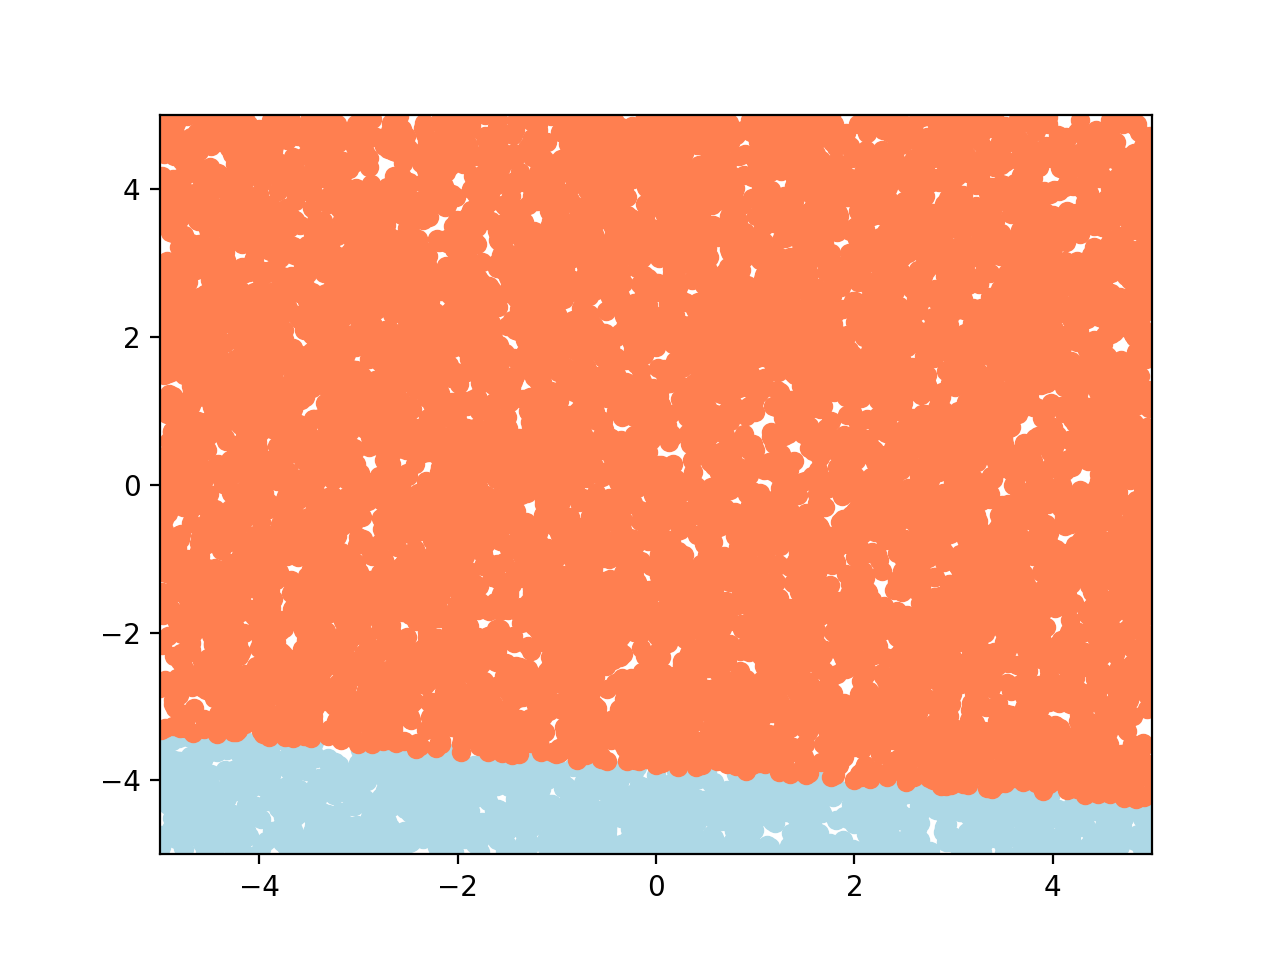
\includegraphics[width=\linewidth]{fig/fig_p23_3.png}
  \caption{$w \in [-0.1, 0.1]$}
\endminipage
\end{figure}


By observation we may tell with the weights $w$ decaying, the output graph becomes more ``linear'' which is better againt overfitting. For color reference, we have \textcolor{cyan}{Output = 1} and \textcolor{orange}{Output = 0}.

% % % % % % % % % % % % % % % % % % % % % % % % % % % % % % % % % %
% % % % % % % % % % % % % % % % % % % % % % % % % % % % % % % % % %
% % % % % % % % % % % % % % % % % % % % % % % % % % % % % % % % % %
\section{Problem 24}


For traditional backpropagation of $n_k$ in $k$-th layer, we have $\frac{\p L}{\p n_k}  = \sum\limits_{k+1 \in \text{Downstream}(n_k)} \frac{\p L}{\p n_{k+1}} \cdot \frac{\p n_{k+1}}{\p n_k}$ assuming there is an edge from $n_k$ to $n_{k+1}$. For the non-feedforward structure the question suggests, $n_k$ will still calculate the above loss, but it will also consider other nodes in the $k$-th layer which it connects to $n_k$. We denotes these nodes as $n_{k_i} = \{n_{k_1}, n_{k_2}, n_{k_3}, ...\}$, where edges like $n_k \to n_{k_i}$ exist. \newline

Since there is no cycle, these $n_{k_i}$ nodes will not connect to any $\text{Downstream}(n_k)$ nodes. So we can just do backpropagation layer by layer and once the above $\sum\limits_{k+1 \in \text{Downstream}(n_k)} \frac{\p L}{\p n_{k+1}} \cdot \frac{\p n_{k+1}}{\p n_k}$ is calculated, we will calculate the loss of $n_{k_i}$ nodes with respect to $n_k$ and add to the loss of $n_k$. Which will give us:

\begin{align*}
    \frac{\p L}{\p n_k}  &= \sum\limits_{k+1 \in \text{Downstream}(n_k)} \frac{\p L}{\p n_{k+1}} \cdot \frac{\p n_{k+1}}{\p n_k} + \sum\limits_{n_{k_i}} \frac{\p L}{\p n_{k_i}} \cdot \frac{\p n_{k_i}}{\p n_k} \\
    \Longrightarrow \frac{\p L}{\p w_{(k-1)k}} &= \frac{\p L}{\p n_k} \frac{\p n_j}{w_{(k-1)k}} \\
    &= \frac{\p L}{\p n_k} \cdot x_{(k-1)k}
\end{align*}

Assume there is a $n_{k-1} \to n_k$ edge.

% % % % % % % % % % % % % % % % % % % % % % % % % % % % % % % % % %
% % % % % % % % % % % % % % % % % % % % % % % % % % % % % % % % % %
% % % % % % % % % % % % % % % % % % % % % % % % % % % % % % % % % %
\section{Problem 25}

\begin{align*}
    P(T = i \mid c_1, \dots, c_N) &= \frac{P(c_1, \dots, c_N \mid T = i)\cdot P(T = i)}{\sum\limits_{i \in \{1, 2, 3\}} P(c_1, \dots, c_N \mid T = i) \cdot P(T = i)} \\
    &= \frac{\prod\limits_{j = 1}^{N} P(c_j \mid T = i) \cdot P(T = i) }{\sum\limits_{i \in \{1, 2, 3\}} \big ( \prod\limits_{j = 1}^{N} P(c_j \mid T = i) \cdot P(T = i)\big ) }
\end{align*}

Since no prior information is exposed, we know $P(T = i) = \frac{1}{3}$ for $i \in \{1, 2, 3\}$. Thus we have:

\begin{equation*}
    P(T = i \mid c_1, \dots c_N) = \frac{\prod\limits_{j = 1}^{N} P(c_j \mid T = i) \cdot \frac{1}{3} }{\sum\limits_{i \in \{1, 2, 3\}} \big ( \prod\limits_{j = 1}^{N} P(c_j \mid T = i) \cdot \frac{1}{3} \big ) }
\end{equation*}



\begin{figure}[!htb]
\minipage{0.32\textwidth}
  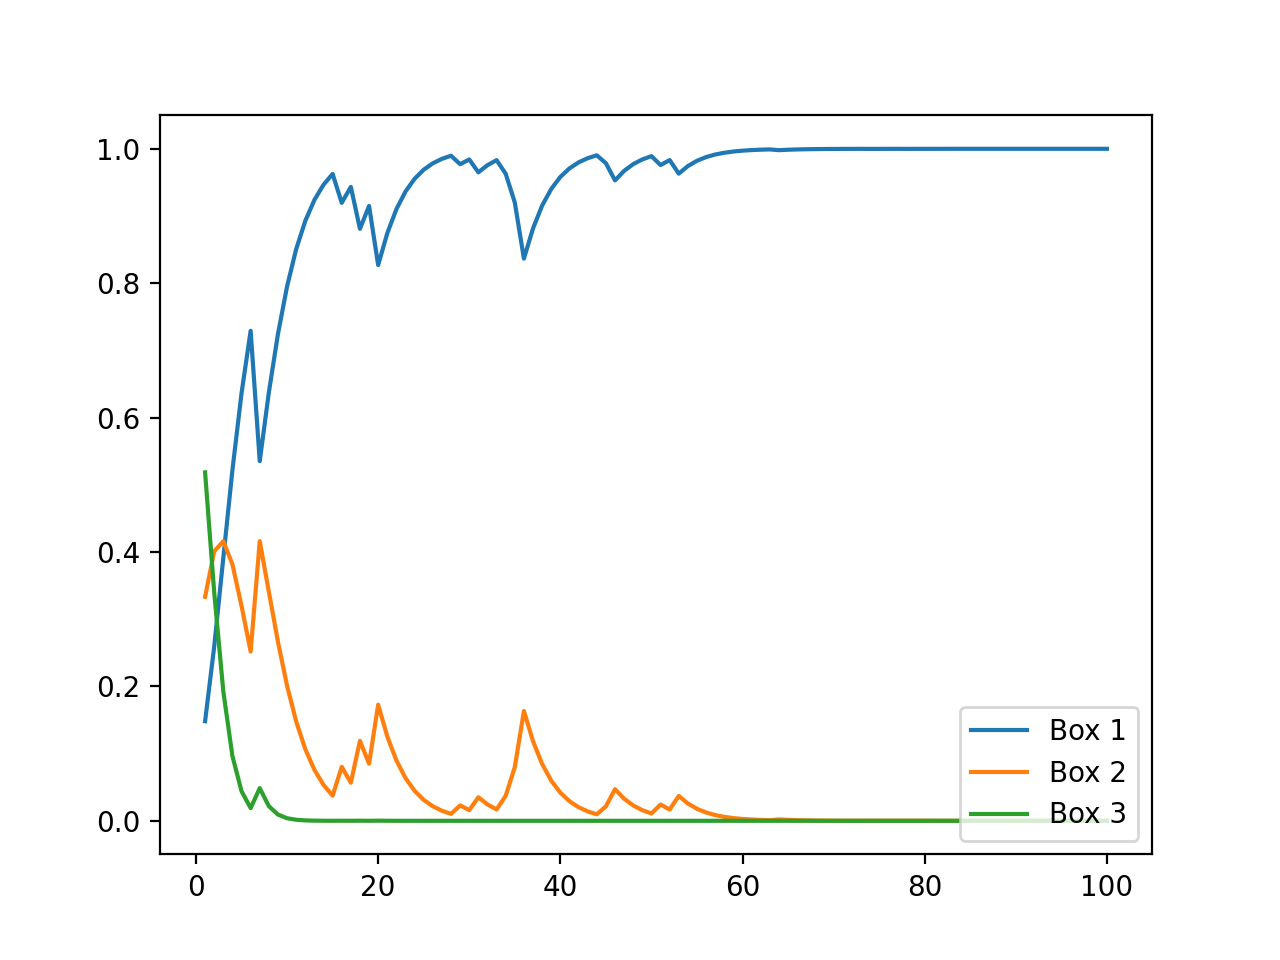
\includegraphics[width=\linewidth]{fig/fig_p25_1.png}
  \caption{Box 1}
\endminipage\hfill
\minipage{0.32\textwidth}
  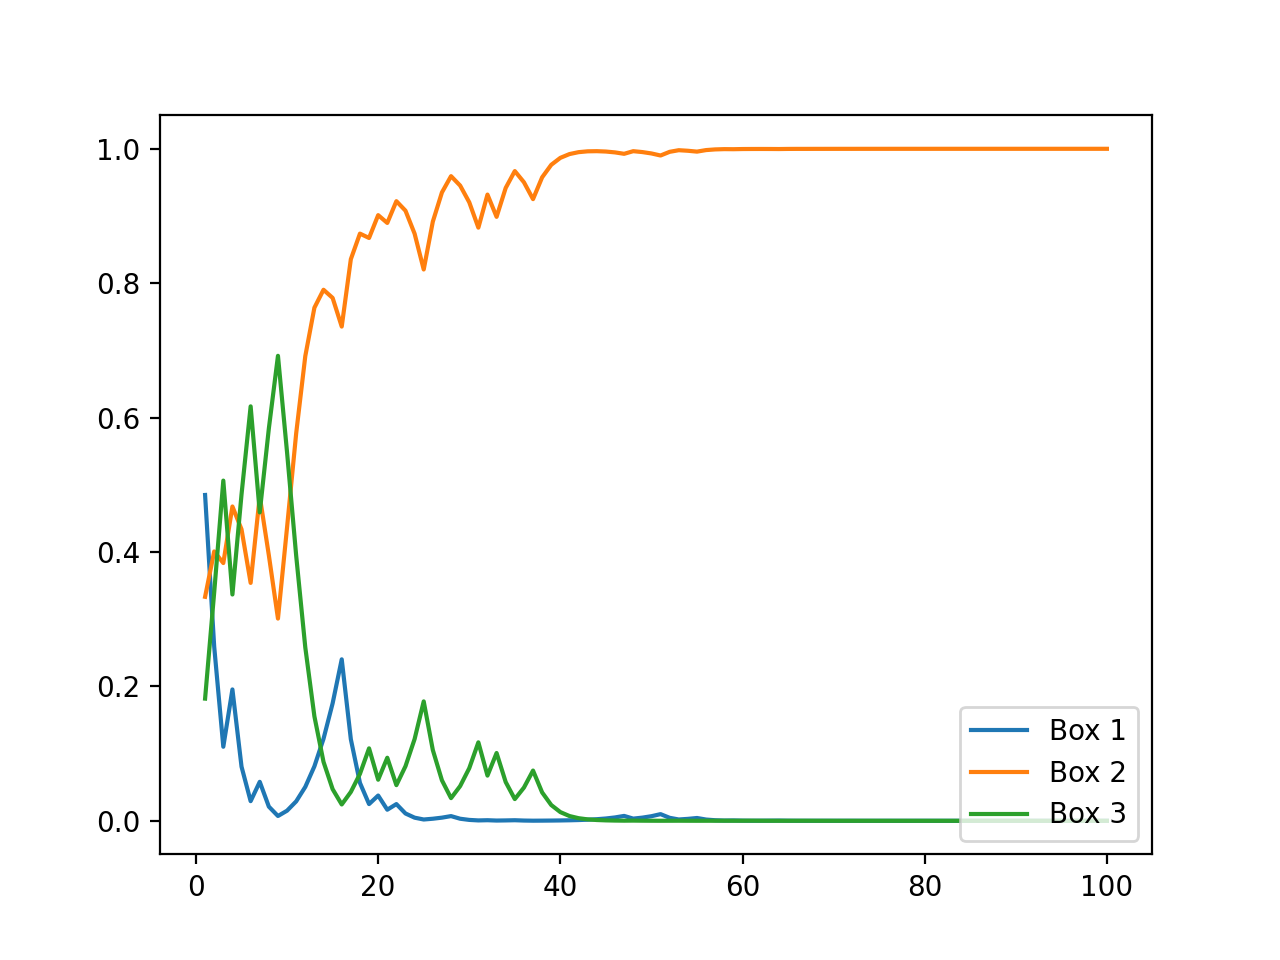
\includegraphics[width=\linewidth]{fig/fig_p25_2.png}
  \caption{Box 2}
\endminipage\hfill
\minipage{0.32\textwidth}%
  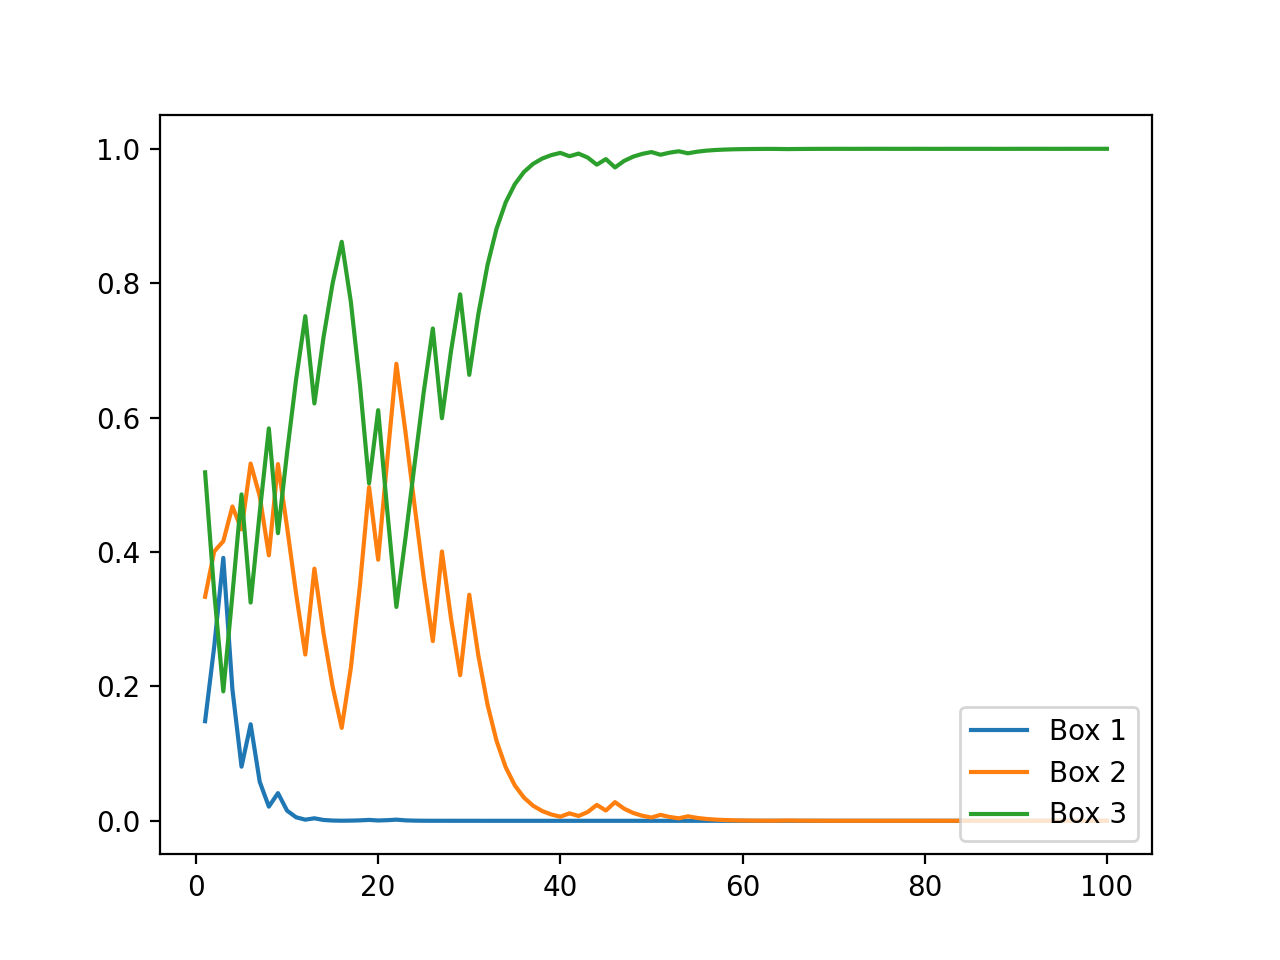
\includegraphics[width=\linewidth]{fig/fig_p25_3.png}
  \caption{Box 3}
\endminipage
\end{figure}


In comparision to \textit{Problem 27}. In \textit{Problem 25} we have all boxes having probablity of $\frac{1}{3}$ instead of $\{0.1, 0.1, 0.8\}$ in \textit{Problem 27}. Reflecting the setting of the questions.

Also it is observable that as more candies were picked, which box we are picking from becomes clear; reflecting the change of decision boundary. Also, boxes with better similiarity (in terms of candy distribution) with the box we picking from will maintain a higher probablity for a longer period time comparing to boxes lack of similiarity to the box we picking from. e.g. When we are picking from Box 1, Box 2 has a higher probablity than Box 3 for a longer period of time before it goes to 0. This is because Box 1 and Box 2 have similar distribution, while Box 3 has the almost opposite distribution to Box 1.

% % % % % % % % % % % % % % % % % % % % % % % % % % % % % % % % % %
% % % % % % % % % % % % % % % % % % % % % % % % % % % % % % % % % %
% % % % % % % % % % % % % % % % % % % % % % % % % % % % % % % % % %
\section{Problem 26}


Similar to pervious question, we have:

\begin{align*}
    P(c_{N+1} = C \mid c_1, \dots, c_N) &= \frac{\sum\limits_{i \in \{1, 2, 3\}} P(c_1, ..., c_N, c_{N+1} = C \mid T = i) }{P(c_1, \dots, c_N)} \\
    &= \frac{\sum\limits_{i \in \{1, 2, 3\}} P(c_1, ..., c_N \mid T = i) P( c_{N+1} = C \mid T = i) }{P(c_1, \dots, c_N)} \\
    &= \sum\limits_{i \in \{1, 2, 3\}} P( T = i\mid c_1, ..., c_N) P( c_{N+1} = C \mid T = i)
\end{align*}

\begin{figure}[H]
\minipage{0.32\textwidth}
  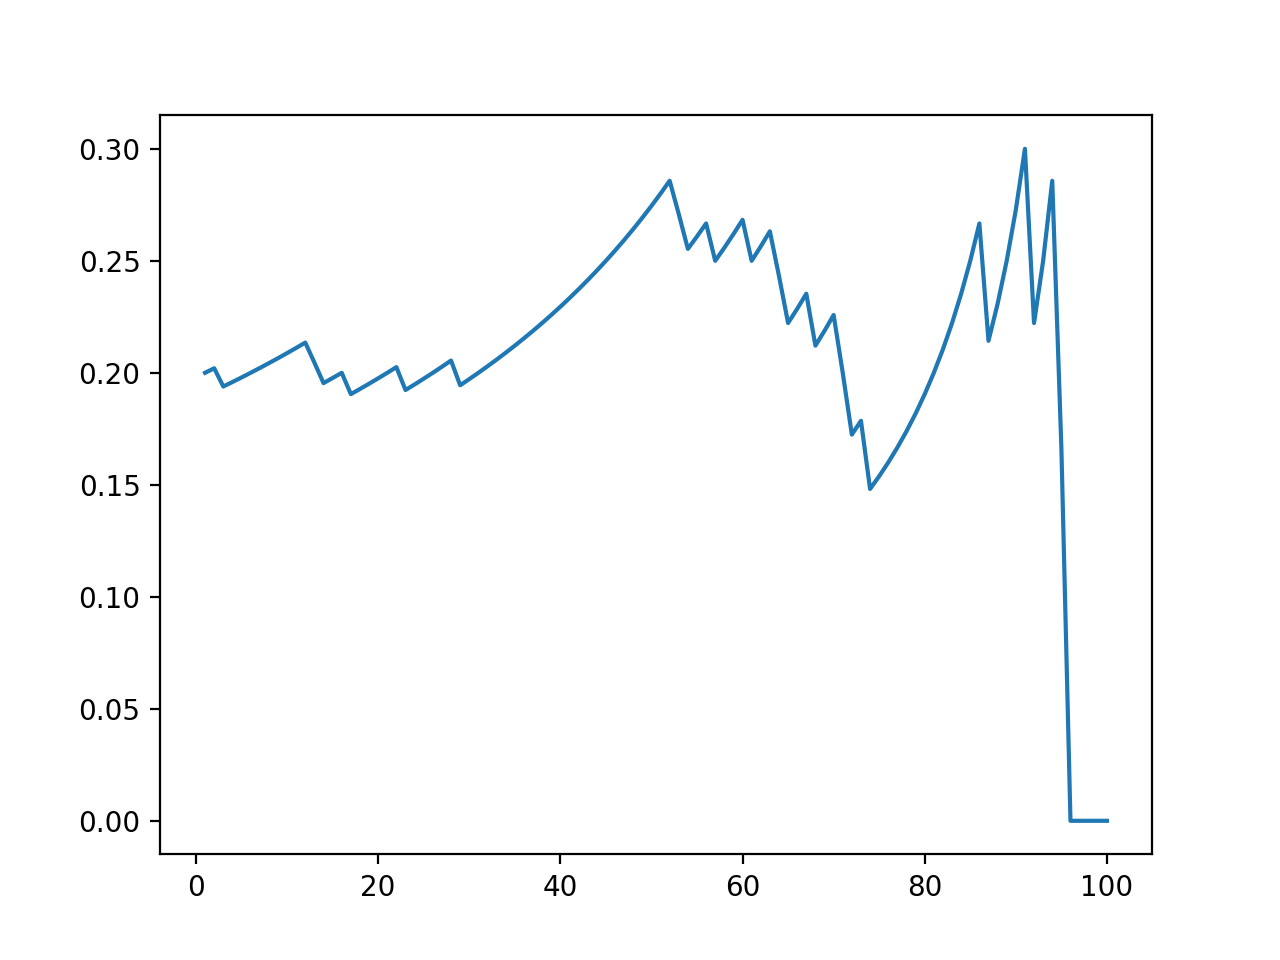
\includegraphics[width=\linewidth]{fig/fig_p26_1.png}
  \caption{Box 1}
\endminipage\hfill
\minipage{0.32\textwidth}
  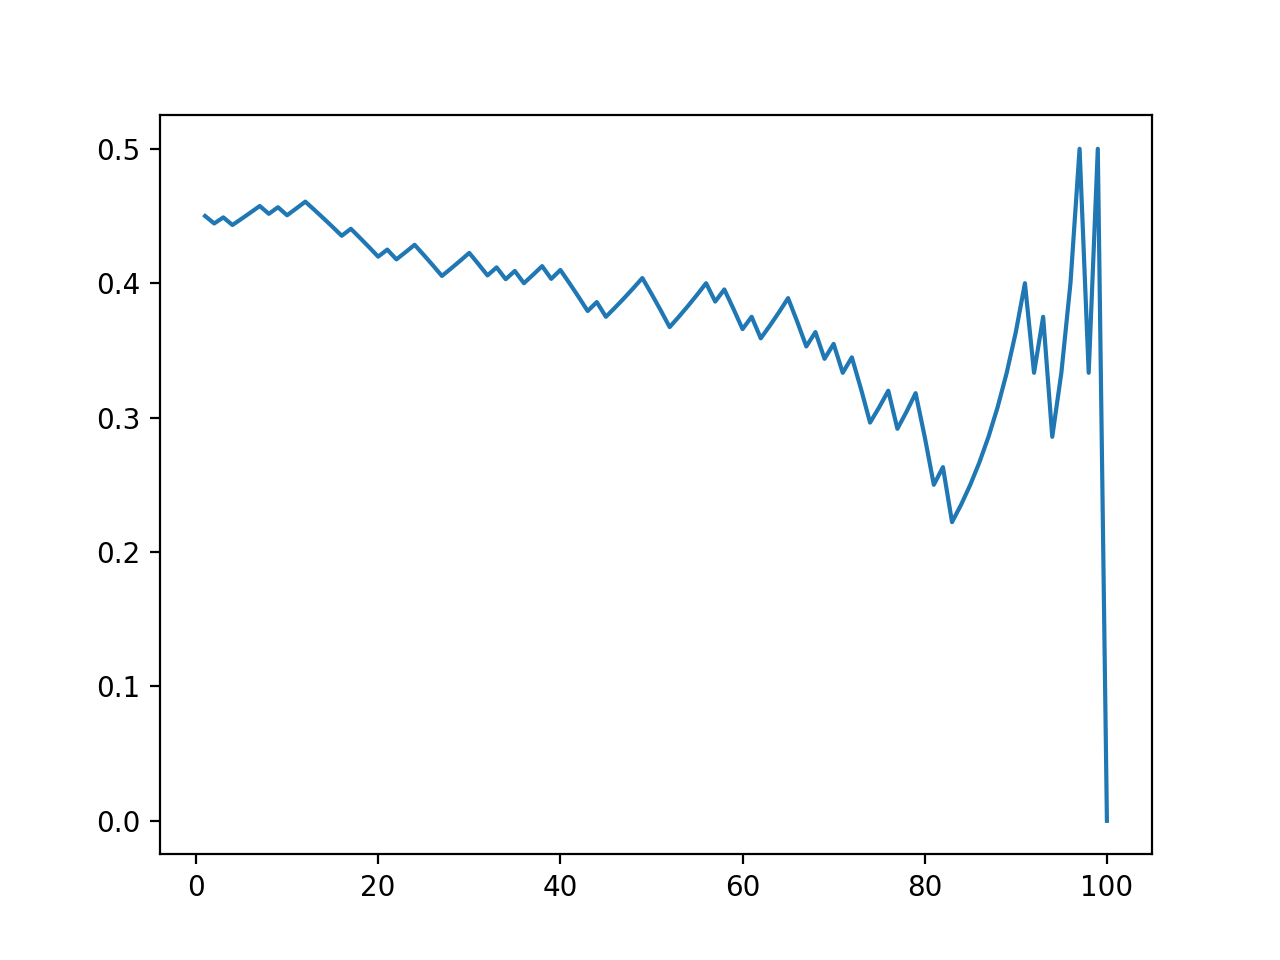
\includegraphics[width=\linewidth]{fig/fig_p26_2.png}
  \caption{Box 2}
\endminipage\hfill
\minipage{0.32\textwidth}%
  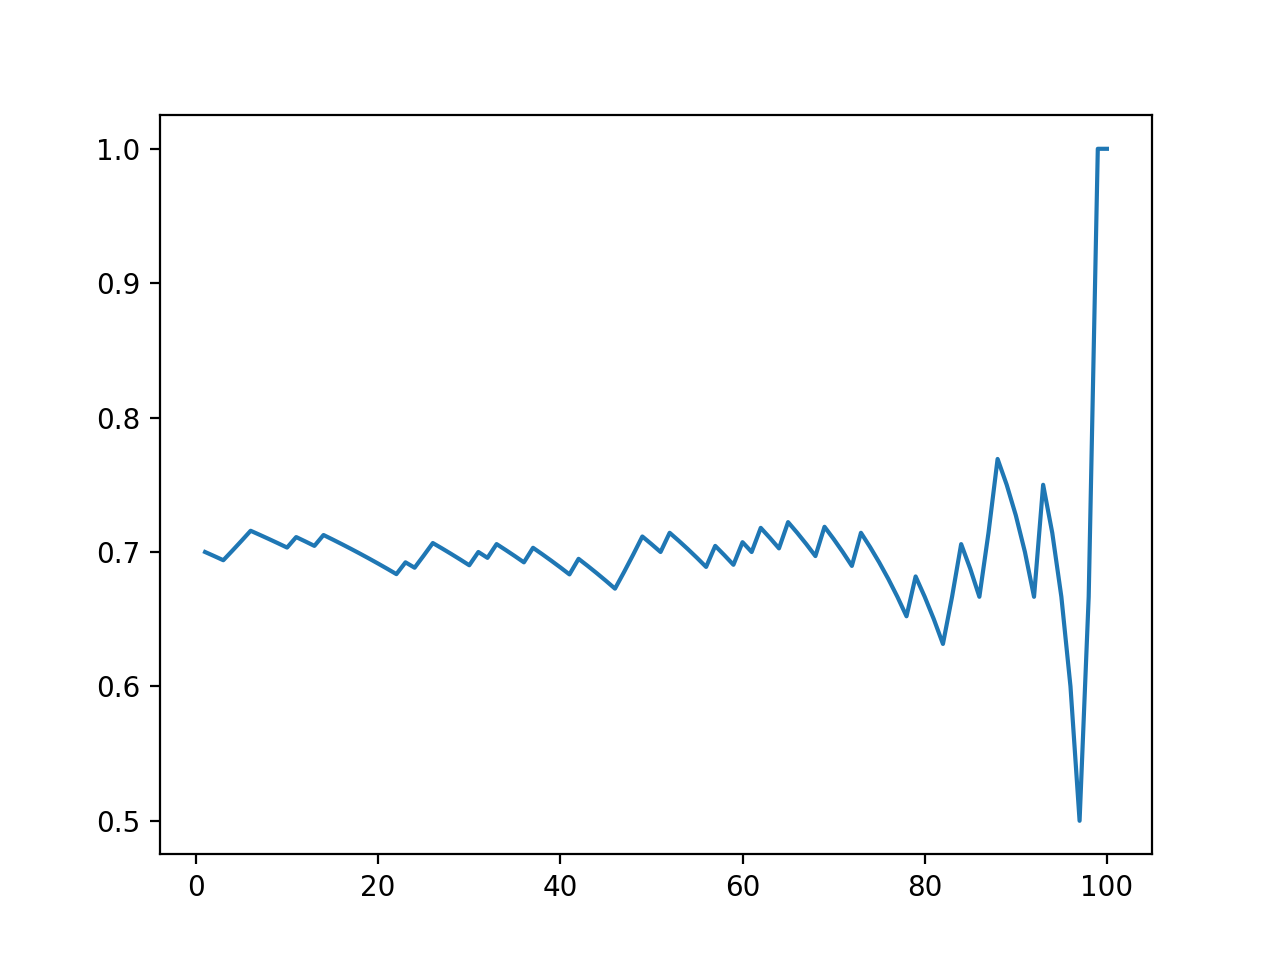
\includegraphics[width=\linewidth]{fig/fig_p26_3.png}
  \caption{Box 3}
\endminipage
\end{figure}

First it is observable that boxes with more $C$ inside has a higher probablity, and every graph starts with the probablity that representing their distribution, reflecting the setting of the problem.

As $N$ is growing, the probablity changes more and more suddenly. This is because candies picked at a later time will have more impact on the probablity -- e.g. the $N+1$ round will either make the probablity be $1$ or $0$ depending on if there is any $C$ left after the $N$-th pick.


% % % % % % % % % % % % % % % % % % % % % % % % % % % % % % % % % %
% % % % % % % % % % % % % % % % % % % % % % % % % % % % % % % % % %
% % % % % % % % % % % % % % % % % % % % % % % % % % % % % % % % % %
\section{Problem 27}


Base on \textit{Problem 25}, we now have $P(T = 1, 2) = 0.1$ and  $P(T = 3) = 0.8$. Now substitute this finding in to the following equation.

\begin{equation*}
    P(T = i \mid c_1, \dots, c_N) = \frac{\prod\limits_{j = 1}^{N} P(c_j \mid T = i) \cdot P(T = i) }{\sum\limits_{i \in \{1, 2, 3\}} \big ( \prod\limits_{j = 1}^{N} P(c_j \mid T = i) \cdot P(T = i)\big ) }
\end{equation*}


\begin{figure}[H]
\minipage{0.32\textwidth}
  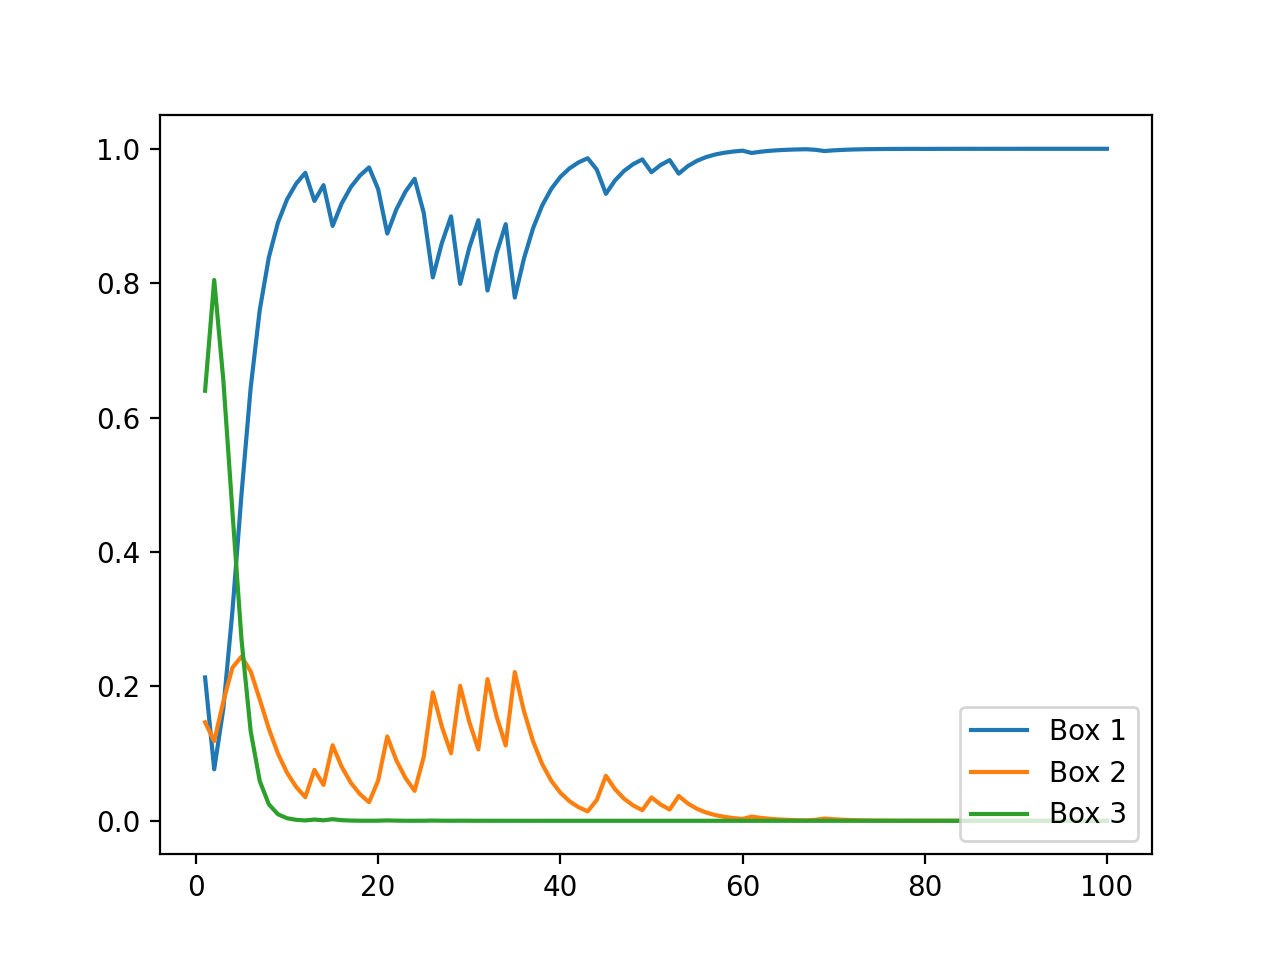
\includegraphics[width=\linewidth]{fig/fig_p27_1.png}
  \caption{Box 1}
\endminipage\hfill
\minipage{0.32\textwidth}
  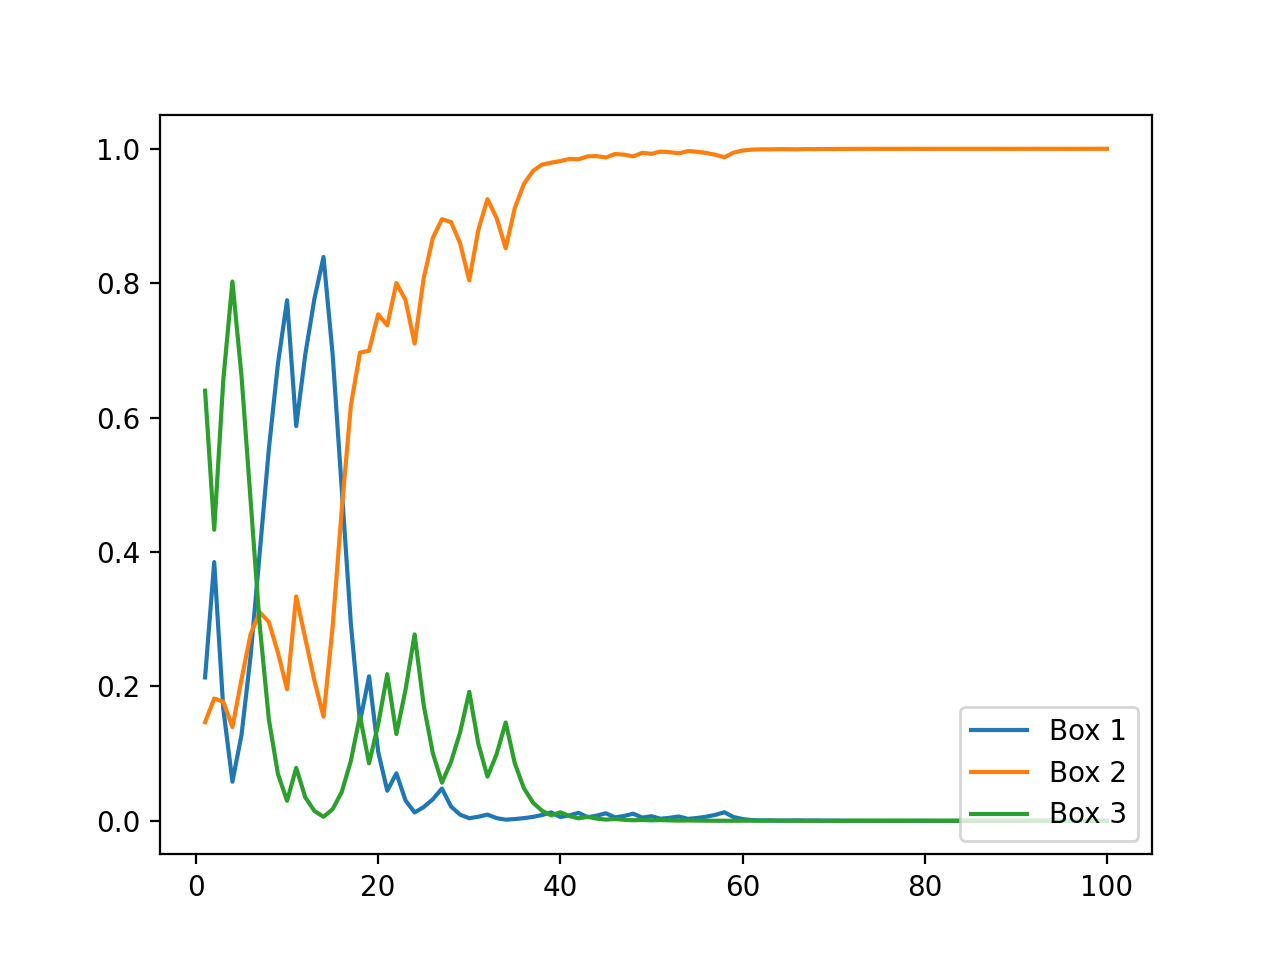
\includegraphics[width=\linewidth]{fig/fig_p27_2.png}
  \caption{Box 2}
\endminipage\hfill
\minipage{0.32\textwidth}%
  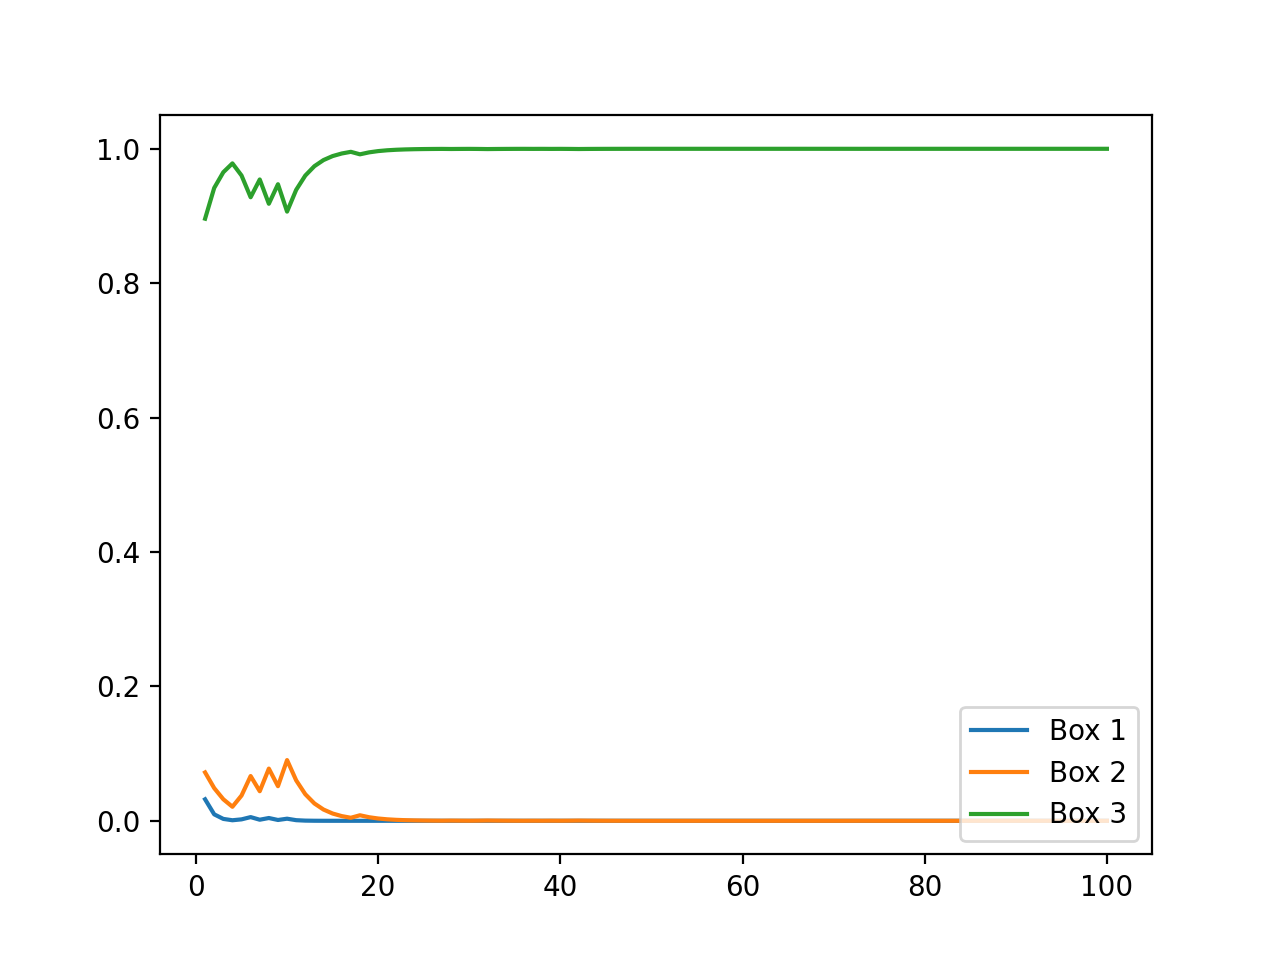
\includegraphics[width=\linewidth]{fig/fig_p27_3.png}
  \caption{Box 3}
\endminipage
\end{figure}

In comparision to \textit{Problem 25}. In \textit{Problem 27} we have each box having an initial probablity of $\{0.1, 0.1, 0.8\}$ instead of $\frac{1}{3}$ in \textit{Problem 25}. Reflecting the setting of the questions.

Also it is observable that as more candies were picked, which box we are picking from becomes clear; reflecting the change of decision boundary. Also, boxes with better similiarity (in terms of candy distribution) with the box we picking from will maintain a higher probablity for a longer period time comparing to boxes lack of similiarity to the box we picking from. e.g. When we are picking from Box 1, Box 2 has a higher probablity than Box 3 for a longer period of time before it goes to 0. This is because Box 1 and Box 2 have similar distribution, while Box 3 has the almost opposite distribution to Box 1.

\end{document}